%%%%%%%%%%%%%%%%%%%%%%%%%%%%%%%%%%%%%%%%%%%%%%%%%%%%%%%%%%%%%%%%%%%%%%%%%%%%%%%%
%2345678901234567890123456789012345678901234567890123456789012345678901234567890
%        1         2         3         4         5         6         7         8

\documentclass[letterpaper, 10 pt, conference]{ieeeconf}  % Comment this line out if you need a4paper

%\documentclass[a4paper, 10pt, conference]{ieeeconf}      % Use this line for a4 paper

\IEEEoverridecommandlockouts                              % This command is only needed if 
                                                          % you want to use the \thanks command

\overrideIEEEmargins                                      % Needed to meet printer requirements.

%In case you encounter the following error:
%Error 1010 The PDF file may be corrupt (unable to open PDF file) OR
%Error 1000 An error occurred while parsing a contents stream. Unable to analyze the PDF file.
%This is a known problem with pdfLaTeX conversion filter. The file cannot be opened with acrobat reader
%Please use one of the alternatives below to circumvent this error by uncommenting one or the other
%\pdfobjcompresslevel=0
%\pdfminorversion=4

% See the \addtolength command later in the file to balance the column lengths
% on the last page of the document

% The following packages can be found on http:\\www.ctan.org
\usepackage{graphics} % for pdf, bitmapped graphics files
\usepackage{epsfig} % for postscript graphics files
\usepackage{mathptmx} % assumes new font selection scheme installed
\usepackage{times} % assumes new font selection scheme installed
\usepackage{amsmath} % assumes amsmath package installed
\usepackage{amssymb}  % assumes amsmath package installed
\usepackage{cite}
\usepackage{cleveref}
\usepackage{comment}

\title{\LARGE \bf
Toward Human-Robot-Teaming for  Robot Navigation Using
Remote  Control, Digital Twin, and  Self-Supervised  Traversability Prediction
}


\author{Trung Kien La$^{1}$ and Eric Guiffo Kaigom$^{1}$% <-this % stops a space
%\thanks{*This work was not supported by any organization}% <-this % stops a space
\thanks{$^{1}$The authors are with the Department of Computer Science \& Engineering,
        Frankfurt University of Applied Sciences, 60318 Frankfurt am Main, Germany, e-mails:
        {\tt\small trung.la@stud.fra-uas.de; kaigom@fb2.fra-uas.de}}%
% \thanks{$^{2}$Eric Guiffo Kaigom is with Deptartment of Computer Science \& Engineering,
% Frankfurt University of Applied Sciences, 60318 Frankfurt am Main, Germany
%         {\tt\small kaigom@fb2.fra-uas.de}}%
}


\begin{document}



\maketitle
\thispagestyle{empty}
\pagestyle{empty}


%%%%%%%%%%%%%%%%%%%%%%%%%%%%%%%%%%%%%%%%%%%%%%%%%%%%%%%%%%%%%%%%%%%%%%%%%%%%%%%%
\begin{abstract}

Collision prediction and avoidance are essential for the autonomous navigation of mobile robots. The prediction of a traversability map is a way to achieve this goal. However, this approach might fail if the prediction model is exposed to novel semantic classes unseen during self-supervised training or  the environment is subject to  highly dynamic motions of living and artificial entities. Included are pedestrians, animals, and  vehicles that the robot can hardly handle. In this paper, we  embrace this challenge by describing the development of a flexible human-robot teaming that leverages the shared control of the robot to accommodate critical situations and allow the human operator to be otherwise engaged. The operator can remotely perceive the surrounding and actively guide the robot as well as participatively share or leave full control to the robot that autonomously moves toward a desired common goal. A situation-aware control signal balances the input of the motion planner of the autonomous robot and the cognitive input of the  remote  operator issued by using affordable  interfaces. %The robot employs a  traversability map to autonomously evolve in unstructured environments. In challenging situations, the human operator can  intervene and seamlessly operate the robot from everywhere by using any web-capable device.  
The human-in-the-loop control is realized through a bidirectional wireless communication between the physical robot and its  digital twin.  The human-robot teaming enhances the likeliness of a safe and successful navigation under dynamic obstacles and enables a navigation without pre-defined goals. The conceptual architecture is introduced and preliminary results are shared.

\end{abstract}


%%%%%%%%%%%%%%%%%%%%%%%%%%%%%%%%%%%%%%%%%%%%%%%%%%%%%%%%%%%%%%%%%%%%%%%%%%%%%%%%
\section{INTRODUCTION}
The navigation of mobile robots in unstructured environments requires the detection, interpretation, and avoidance of obstacles.  
Self-supervised learning can be leveraged to train  models that predict the traversability map from RGB and depth images data forwarded as inputs to a motion planner to generate collision-free motions to a desired location \cite{wayfaster,wayfast,leung2022hybrid,endo2024benchnav}. 
Even though traversability values can incorporate the semantics of obstacles beyond their standard geometric detection, their reliability can drop in dynamic and previously unseen environments \cite{frey2024roadrunner,muhamad2024robust} where people or other entities exhibit a high motion dynamics, too. Furthermore, pivotal parameters are often overlooked by these models. Included are the battery state of charge (SoC) and engine temperatures of the robot that are equally important to predict a feasible and safe navigation. It is therefore common for robots to be  teleoperated by a human operator \cite{huang2024evaluation,husky}. However, teleoperation might require the constant attention of the operator, which prevents the operator from accomplishing other (e.g., rescue) tasks or being engaged otherwise at the same time.


\begin{figure}[t]
	\centerline{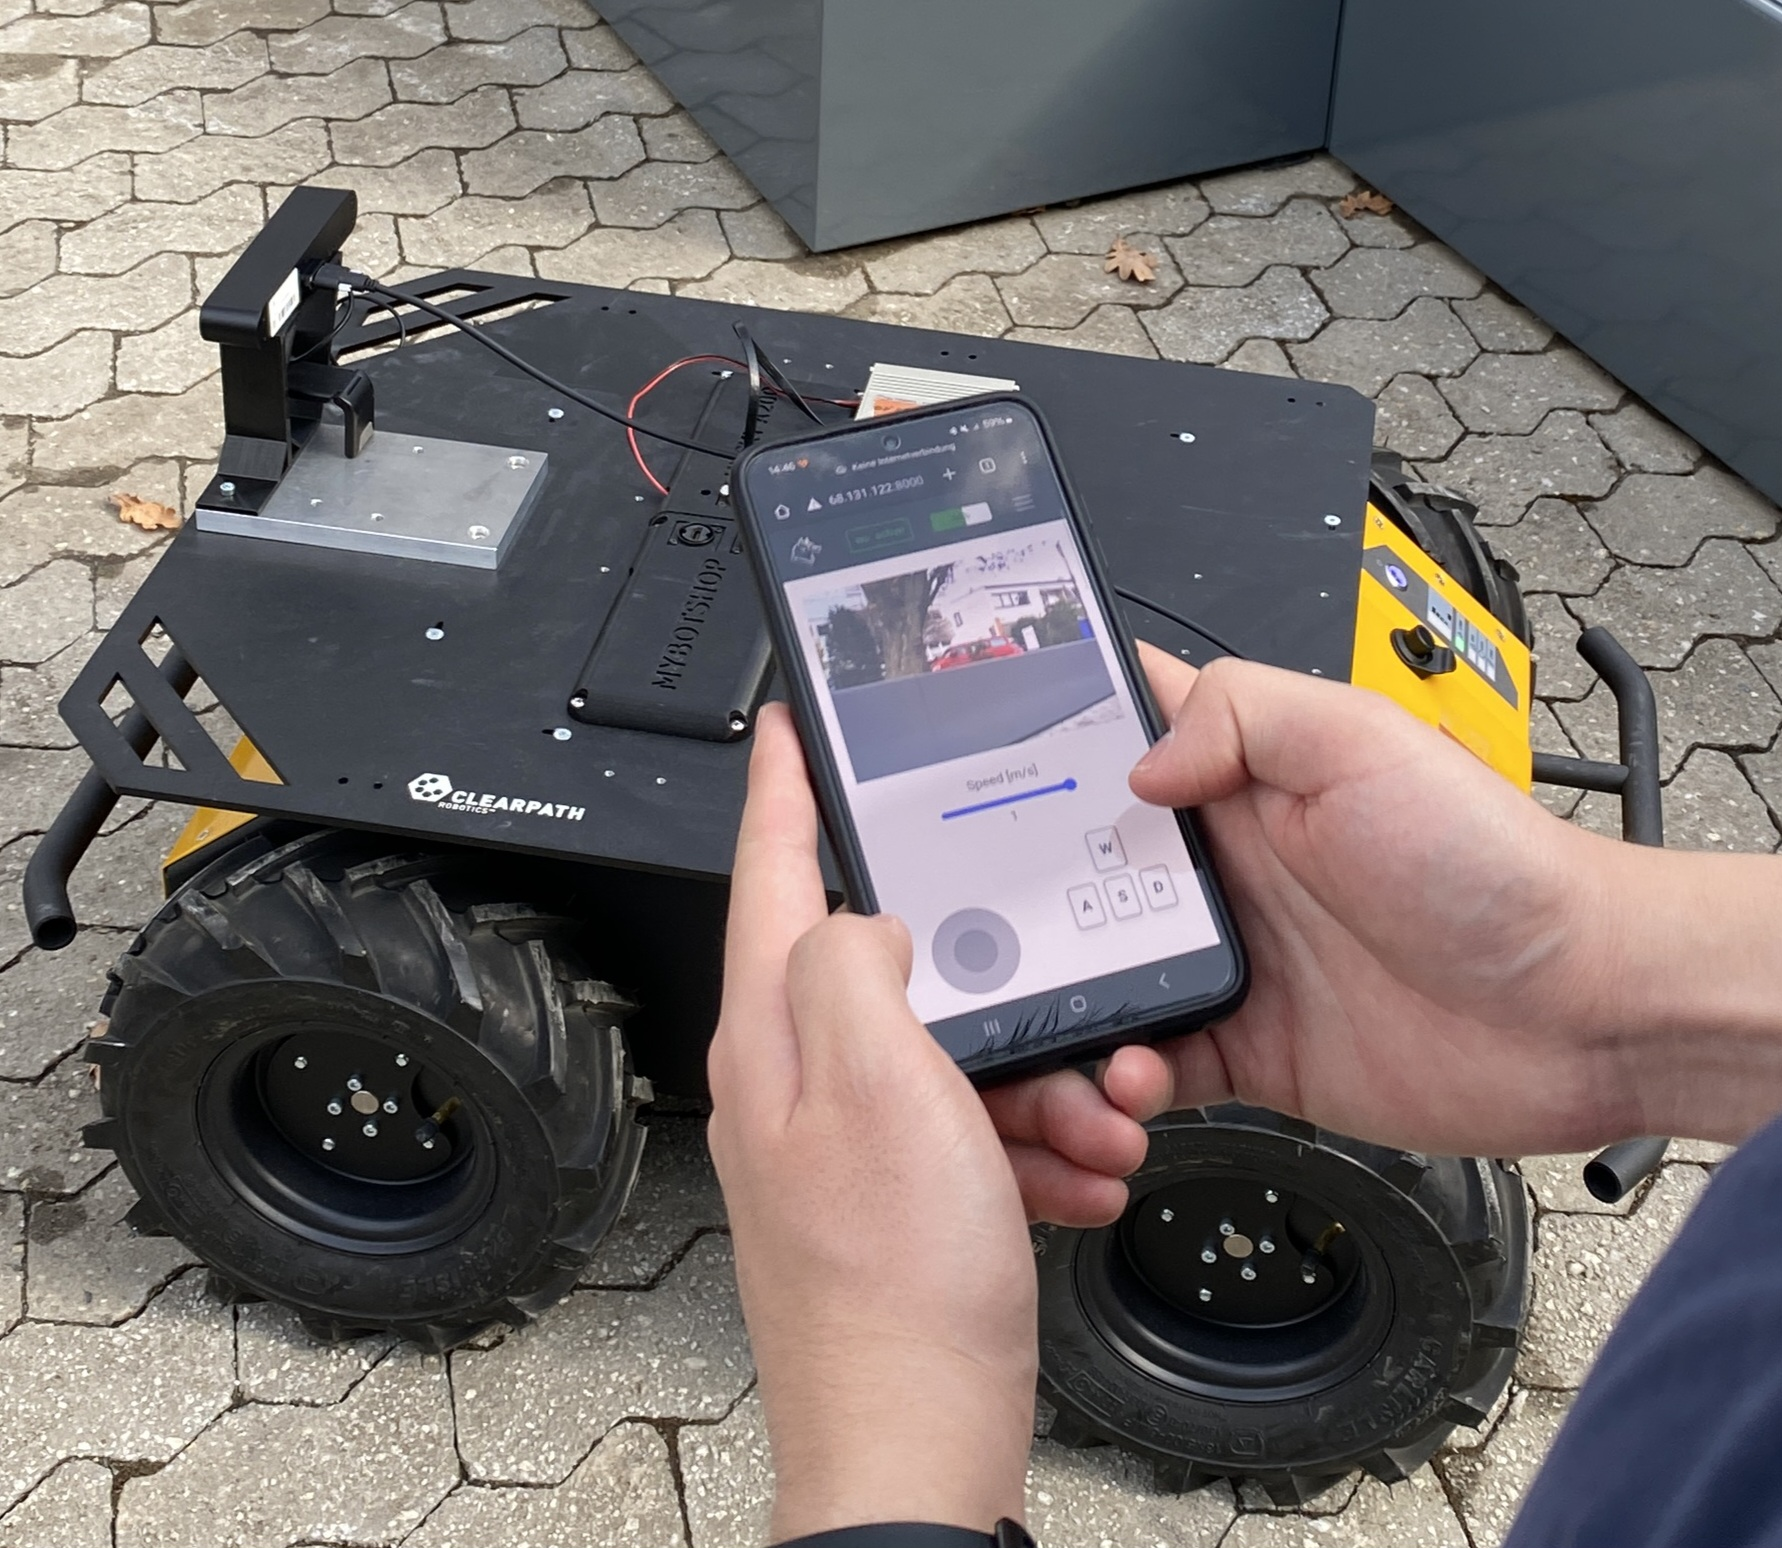
\includegraphics[width=0.9\columnwidth]{images/galaxycontrol.jpg}}
	\caption{Human-robot-teaming for mobile robot navigation.}
	\label{fig:galaxycontrol}
\end{figure}


In this paper, we strive to relax this constraint. We focus on a loosely-coupled collaborative interaction between a  robot and its remote operator  with a customizable level of human intervention and robot autonomy during  safe robot navigation. On the one hand, experienced situation understanding and  supervision skills of humans help remotely guide and assist the robot in challenging situations. Uncertainties from unseen classes are expected to be  accommodated and transformed into advantages. On the other hand, a robot's autonomous navigation abilities allow its human operator to carry out additional tasks while the robot moves toward a desired location. Between full guidance and full autonomy, cognitive skills of the human operator (e.g., perception, empathy, anticipation, etc.) are being superimposed on top of obstacle-aware commands of the motion planner of the robot to  adjust the behavior of the robot and further upskill its navigation. This collaboration is likely to raise the success rate of  navigation by combining the skillsets of humans and robots \mbox{in a seamless and dynamic way.}



Toward this end, we  provide the robot operator with a web-based graphical unit accessible from most devices (see Fig. \ref{fig:galaxycontrol}). The unit interfaces the robot through its digital twin, reflects the perception of the internal state of the robot and its surroundings as live video streams, visualizes its critical data, and offers multiple control options at e.g. velocity level. We strive to sum  velocity signals from the motion planer of the mobile robot and the graphic unit used by the operator to realize shared control \cite{phri} of the robot that fosters human-robot-teaming. To this end, the  autonomous behavior of the robot and amount of human interventions are  balanced by an arbitration factor that depends upon the traversability map of the robot in real-time. Security aspects such as login and persistent data storage via a database are taken into account. 









\section{RELATED WORK}

Virtual-reality (VR) based interactions have been recently proposed in \cite{huang2024evaluation} for the intuitive oversight of robot teams. The VR interface supports the reconstruction of pre-recorded 3D models and real-time capture of scenes, similarly to our work. However,  traversability was not considered to semantically handle obstacles. There are several web-based apps that have been developed for ROS robots such as the Husky Unmanned Ground Vehicle (UGV) by Clearpath (see Fig.\ref{fig:galaxycontrol}) \cite{husky}. These applications are often simple, intuitive and inexpensive as they control virtual robots and are suitable for ROS novices.
They are based on the Rosbrigde protocol, which provides an interface between ROS and web apps via a WebSocket connection\cite{kapic,dinodi,rosbridgeOkState,rosbridgeSuite}.
The protection of the app or the visualization and storing of parameters such as the real battery SoC play an increasingly critical role for autonomous robots.
Hence, we implement a database and visualize ROS data that the Husky provides via its topics.  Further implementations are described in \ref{sec:framework}.
Operators have been provided in \cite{walker2024cyber} with egocentric and exocentric 3D perspectives on robots. However, shared control to balance control modes between a planner and operator was omitted. 





\section{Web-Based Interface for remote operator}
\label{sec:framework}

\begin{figure}[b]
	\centerline{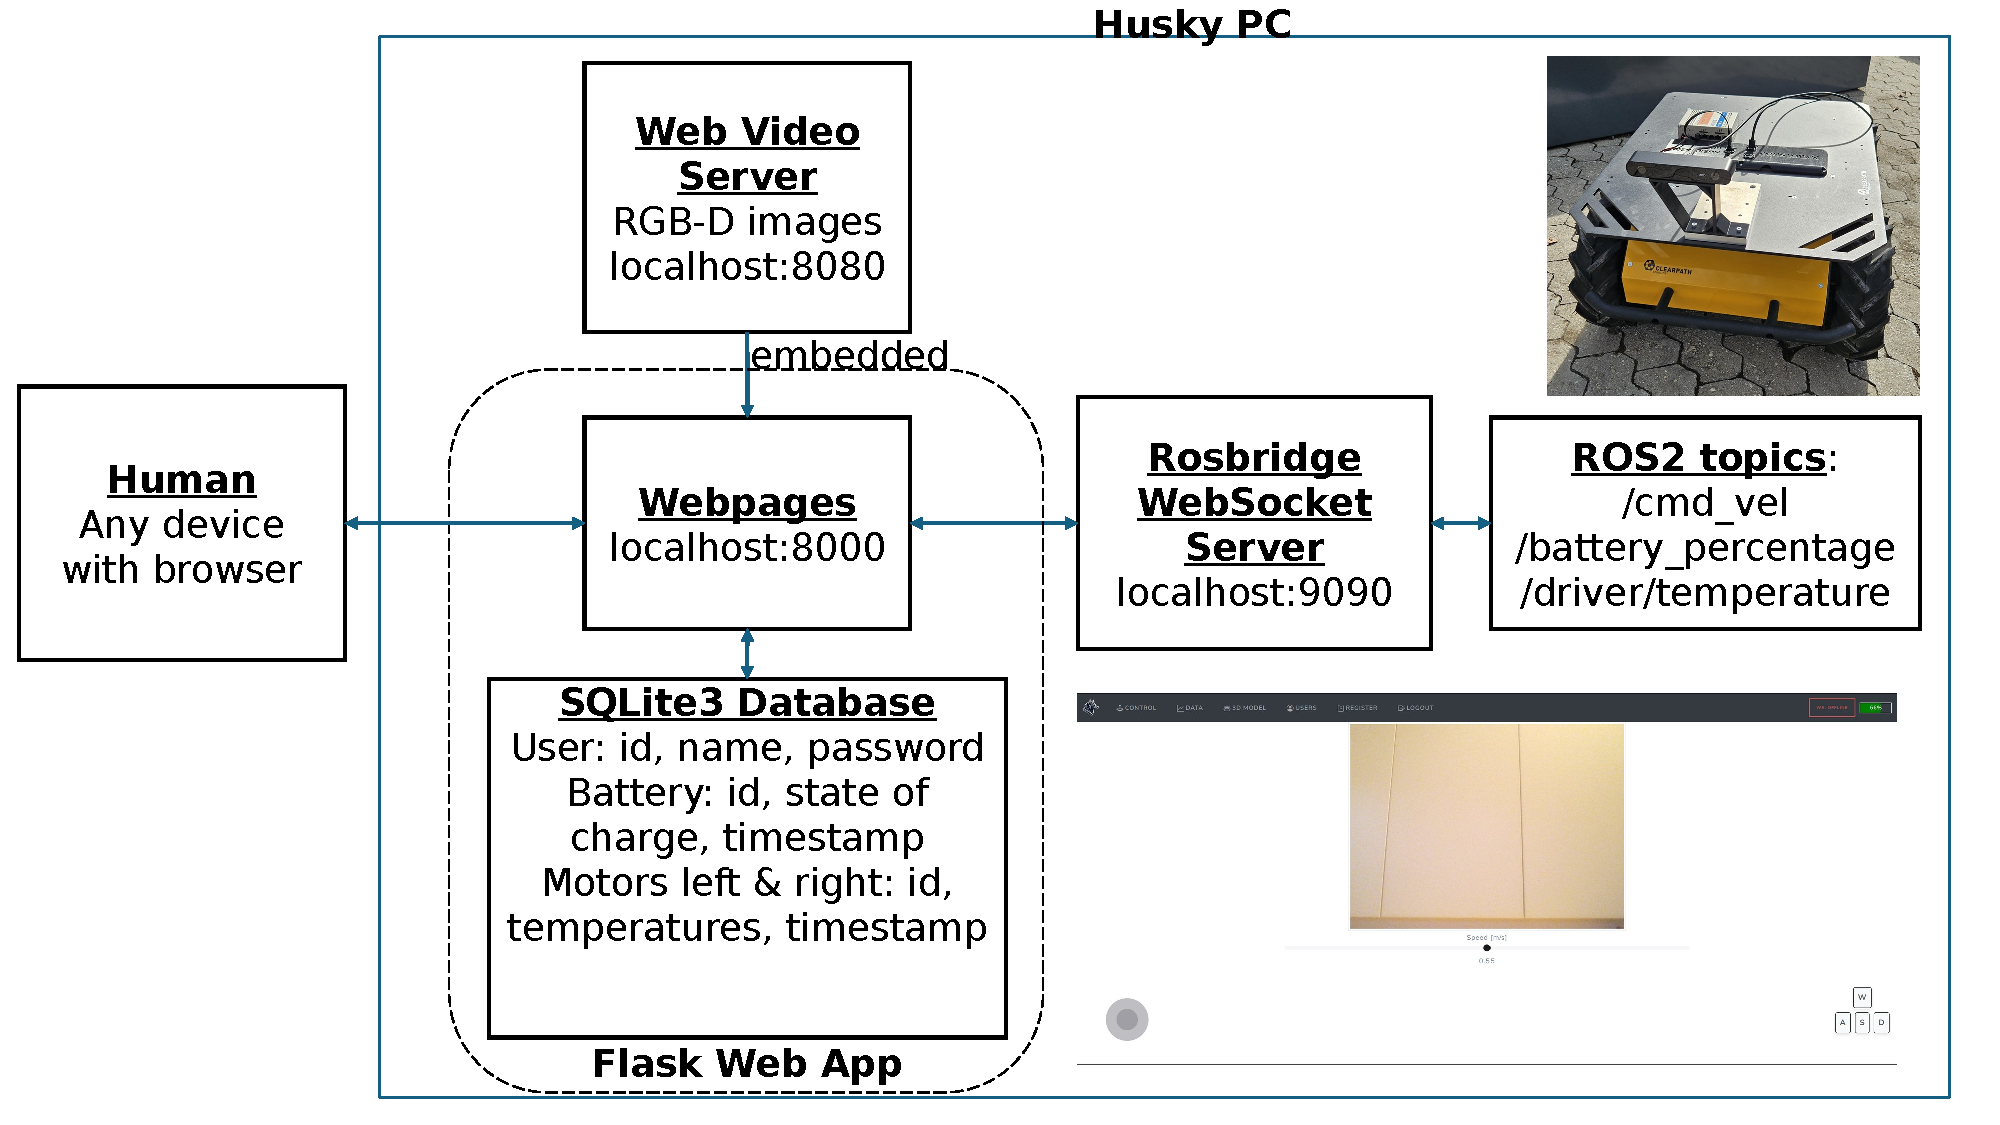
\includegraphics[width=8.5cm]{images/ROS_Web_App_Architecture.pdf}}
	\caption{Backend architecture of the web app and tools used. The digital twin (bottom right) reflects hidden and hardly accessible motor and battery states to assess and predict the feasibility of planned motions.}
	\label{fig:userapp}
\end{figure}



The web framework is based on Flask \cite{flask} and is used to control and monitor the Husky, which runs on ROS2 Humble and is platform-independent.
Bidirectional communication between human and robot is provided by the rosbridge\_suite package \cite{rosbridgeSuite}.   
% Due to the web-based approach, all devices with a browser can access the app, provided they are in the same local network as the robot.
A web-based approach allows the app to be accessible from any device that is in the same local network as the robot.
Fig. \ref{fig:userapp} shows the backend architecture, ROS packages, and other relevant information which were leveraged for developing the framework. 
A twist message, which consists of angular and linear velocity, can be sent from the webpage (frontend) via e.g. 
an intuitive virtual joystick to the /cmd\_vel topic of the robot to teleoperate it. Visualized otherwise invisible ROS data about the robot (see Fig. \ref{fig:overviewplots} and \ref{fig:userapp}) offer a digital twin for decision support.



\subsection{Control panel}
The control panel in Fig. \ref{fig:clip} shows a live image stream of a Zed2i camera attached on the Husky. Above the camera image, a navigation bar is located. i
Below the camera image are two control elements, a virtual joystick and virtual keyboard buttons, which serve as a means for controlling the Husky.
The arrangement of the control elements was chosen to reflect the natural hand position when operating the displays.
Additionally, the Husky can be controlled with a physical keyboard when the operator has access to the control panel, which is protected by a login system. Keyboard control can be helpful in situations where finer precision is required compared to the joystick.
Other elements such as the battery SoC and the WebSocket connection are embedded in the navigation bar to ensure that the operator is always informed of the robot's energy and connection status to assess the feasibility of planned navigation.
% about the energy and connection status of the robot to assess the feasibility of a planned navigation.







\begin{figure}[b]
	\centerline{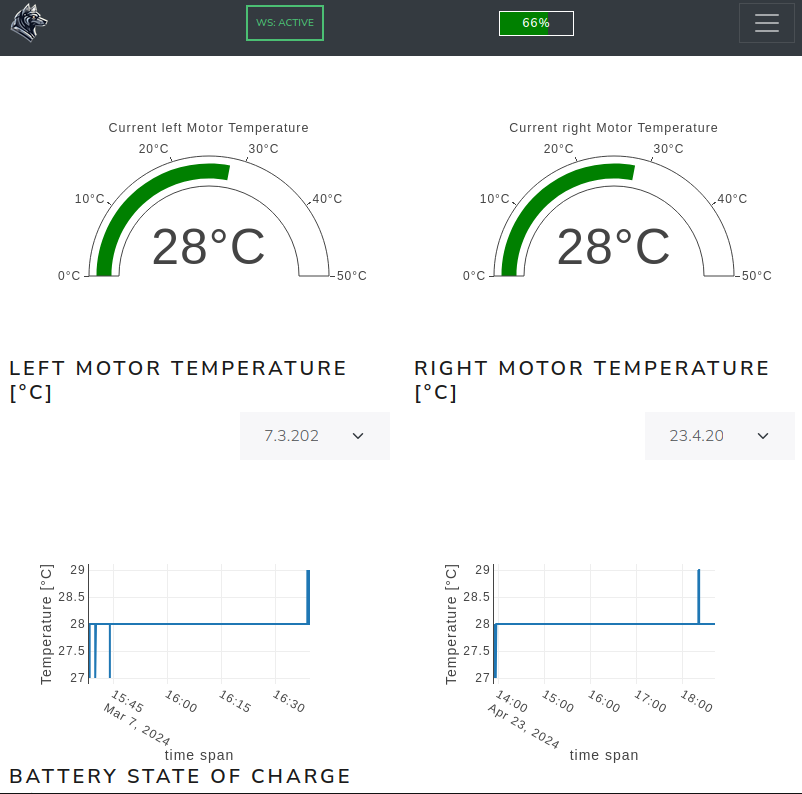
\includegraphics[width=0.8\columnwidth]{images/tabletdatasm.png}}
	\caption{Data panel as component of the digital twin (monitoring service$\slash$interface layer in Fig. \ref{fig:DT}). Sensed left and right motor temperatures are presented live as gauges. Historic data managed via a SQLite database.}
	\label{fig:overviewplots}
\end{figure}

\subsection{Data panel}
The data panel in Fig. \ref{fig:overviewplots} shows critical live robot data such as the left and right motor temperatures as gauges. 
Furthermore, the temperatures and the battery SoC are shown in diagrams with time progression. 
The data for the visualization is provided by an SQLite database, which in turn reads the data from the respective ROS topics of the Husky. 
It is possible to select and visualize historical logs of single days in the diagrams and snapshots can be taken if required.



%\begin{figure*}[htbp]
%    \centerline{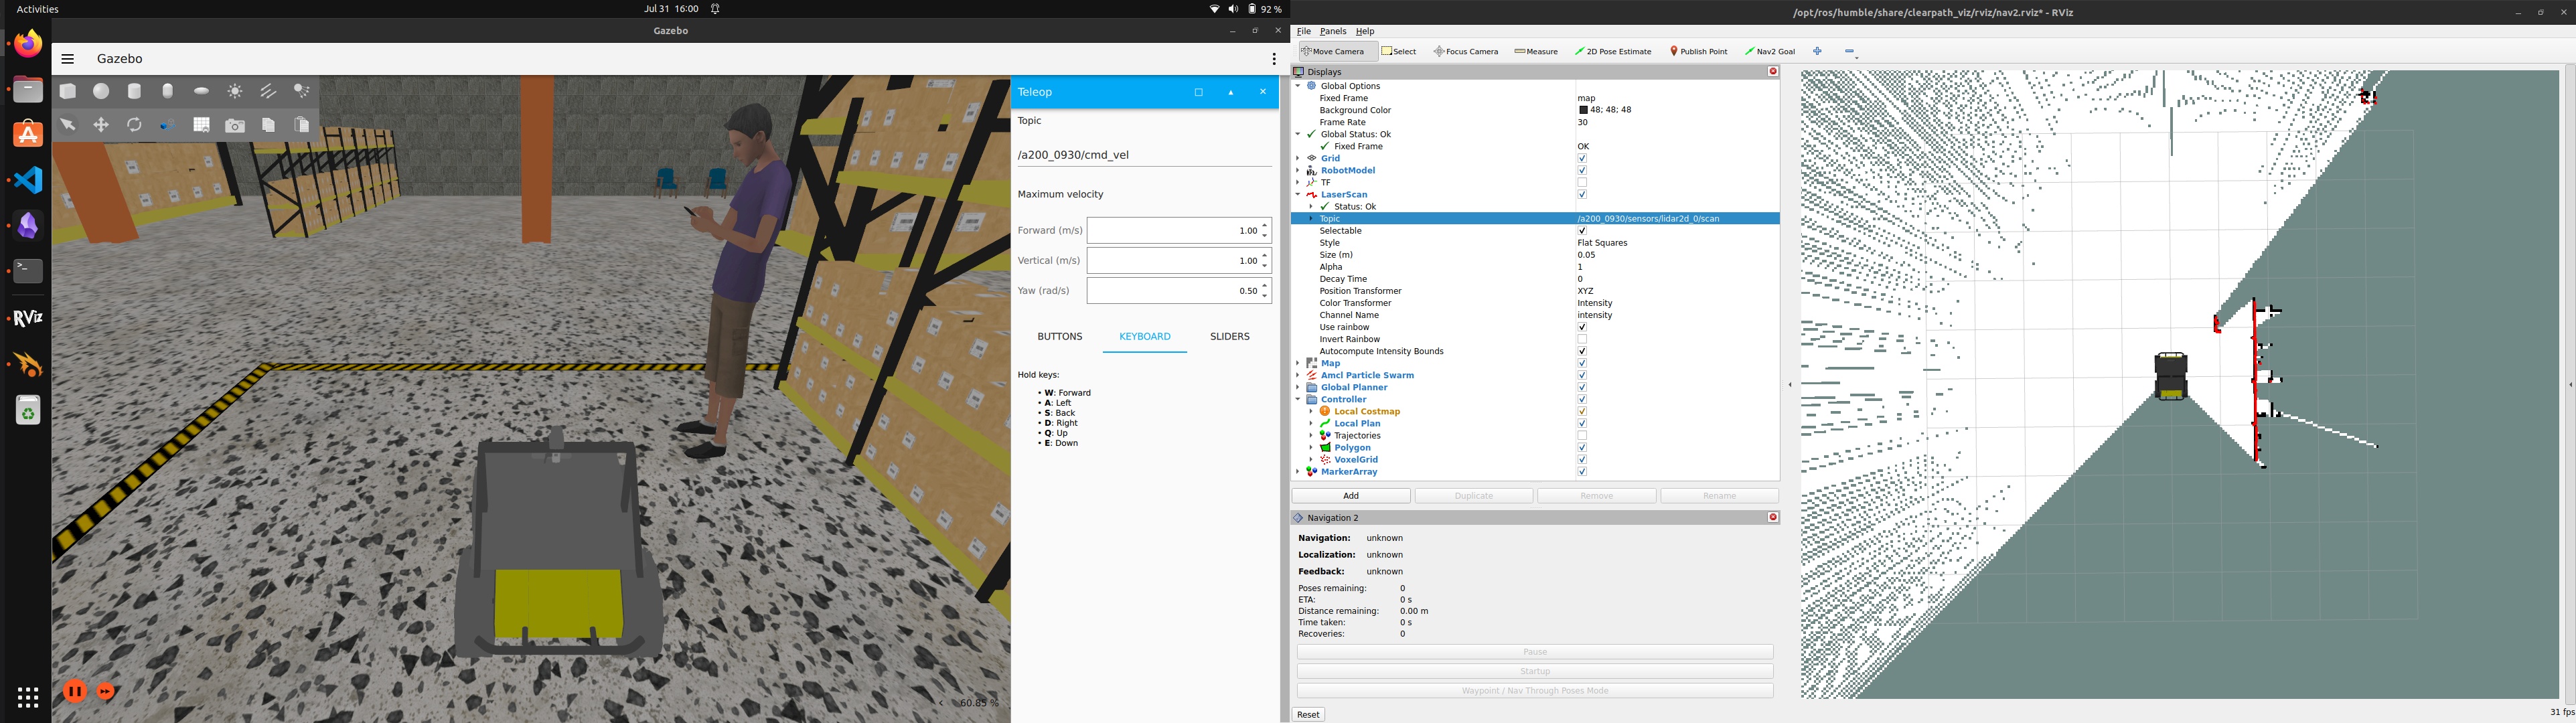
\includegraphics[width=16.35cm]{images/sim_husky_mapping.png}}
%    \caption{Indoor map generation with LiDAR (SLAM) in a simulation environment.}
%    \label{fig:huskymapping}
%\end{figure*}



\subsection{Additional features of the operator interface }
A user login system is implemented for privacy preservation  and security purposes. A six-layer digital twin architecture (see Fig. \ref{fig:DT}) supports the monitoring, 3D visualization, and control of the robot. Robot perception and supervision are thereby facilitated. 
A specially developed OPC UA server keeps the framework open, semantically interoperable, scalable, and industry-relevant. The server exposes e.g. current states of manipulators, mounted on the Husky, in real-time. These data can be stored in the SQLite database and visualized on the web interface, which therefore acts as a multi-modal immersive interface. Bootstrap, a frontend framework, was leveraged to facillitate responsive web design \cite{bootstrap}. 
This allows control elements and data visualizations to be optimally displayed on mobile or desktop devices and ensures that the operator experiences a pervasive, contextualized, and personalized \mbox{overview and collaboration with the robot.}

\begin{figure}[t]
	\vspace{0.2cm}
	\centerline{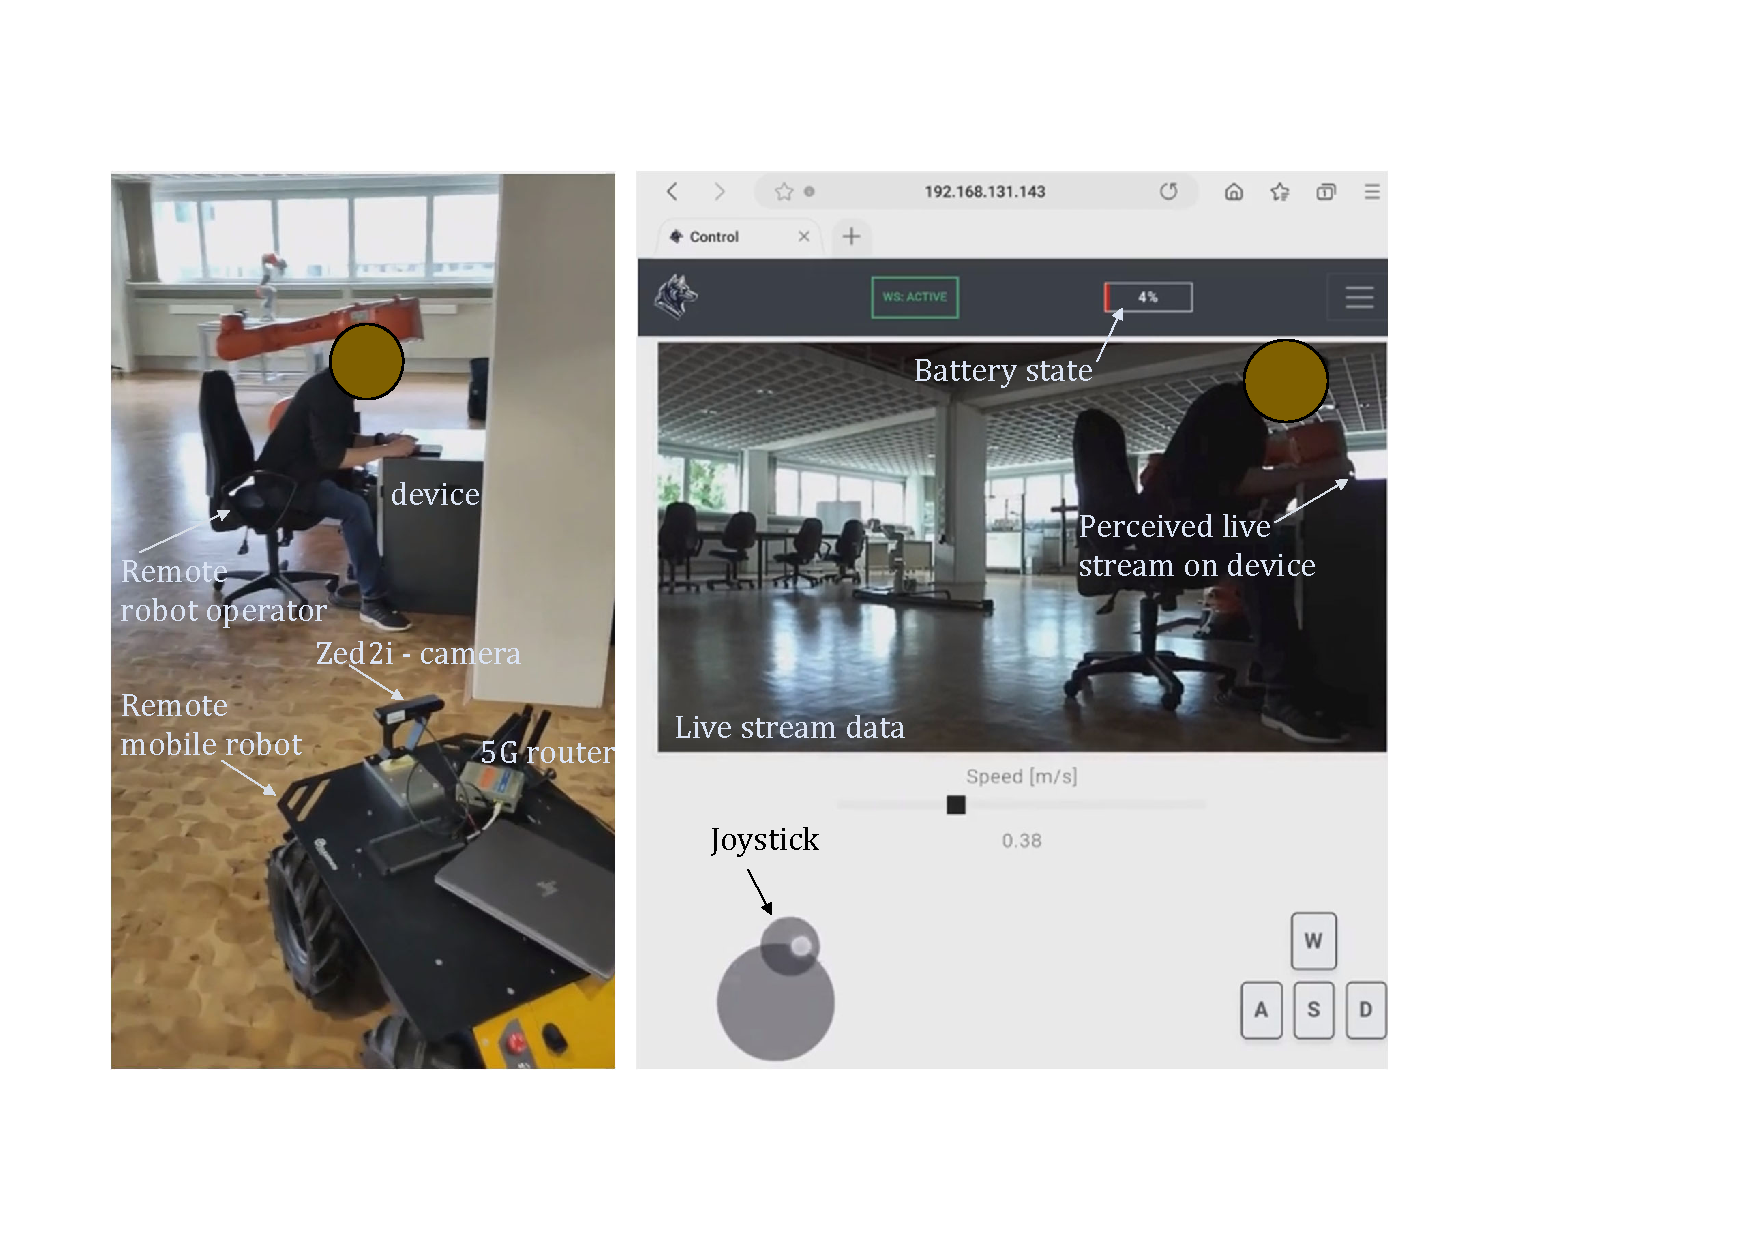
\includegraphics[height=0.7\columnwidth]{images/telehusky.pdf}}
	\caption{Remote control (top left) of the Husky robot (bottom left) in real-time via the web interface with a virtual joystick, a speed slider and  live camera images (top right). The battery state helps predict motion feasibility.}
	\label{fig:clip}
\end{figure}


\section{Multi-modal Remote Control of the Robot}
We strive to offer three modalities (see Fig. \ref{fig:statemachine}) for the remote control of the mobile robot in our ongoing work. During  full control, the remote operator actively guides the robot. Interface details and  results on this control mode are provided in  \cref{sec:framework}. Its core advantage is the direct usage of experienced human skills and knowledge to yield a thoughtful robot behavior. Since the operator might be occupied with the completion of  tasks with a higher priority, the second autonomous control mode differs  in the sense that the path planner of the robot aims at achieving safe motions and the operator does not intervene. To this end, the path planner is provided with traversability values from a prediction model trained by using self-supervised learning \cite{wayfaster}. A semantic understanding of the terrain  is incorporated in these values. Unlike geometrical approaches, semantic obstacle awareness facilitates an intelligent estimation of traversability in the presence of  different properties of objects. While a stiff wall and tall grass can be geometrically identical, the latter is traversable and the former is not. As human intervention becomes critical, the third shared control mode balances previous schemes by combining human and machine intelligence. Flexibility from autonomy and acumen from supervision are likely to enlarge the range of supported applications and enhance the operator experience in practice.




\begin{figure}[t]
	\vspace{0.2cm}
	\centerline{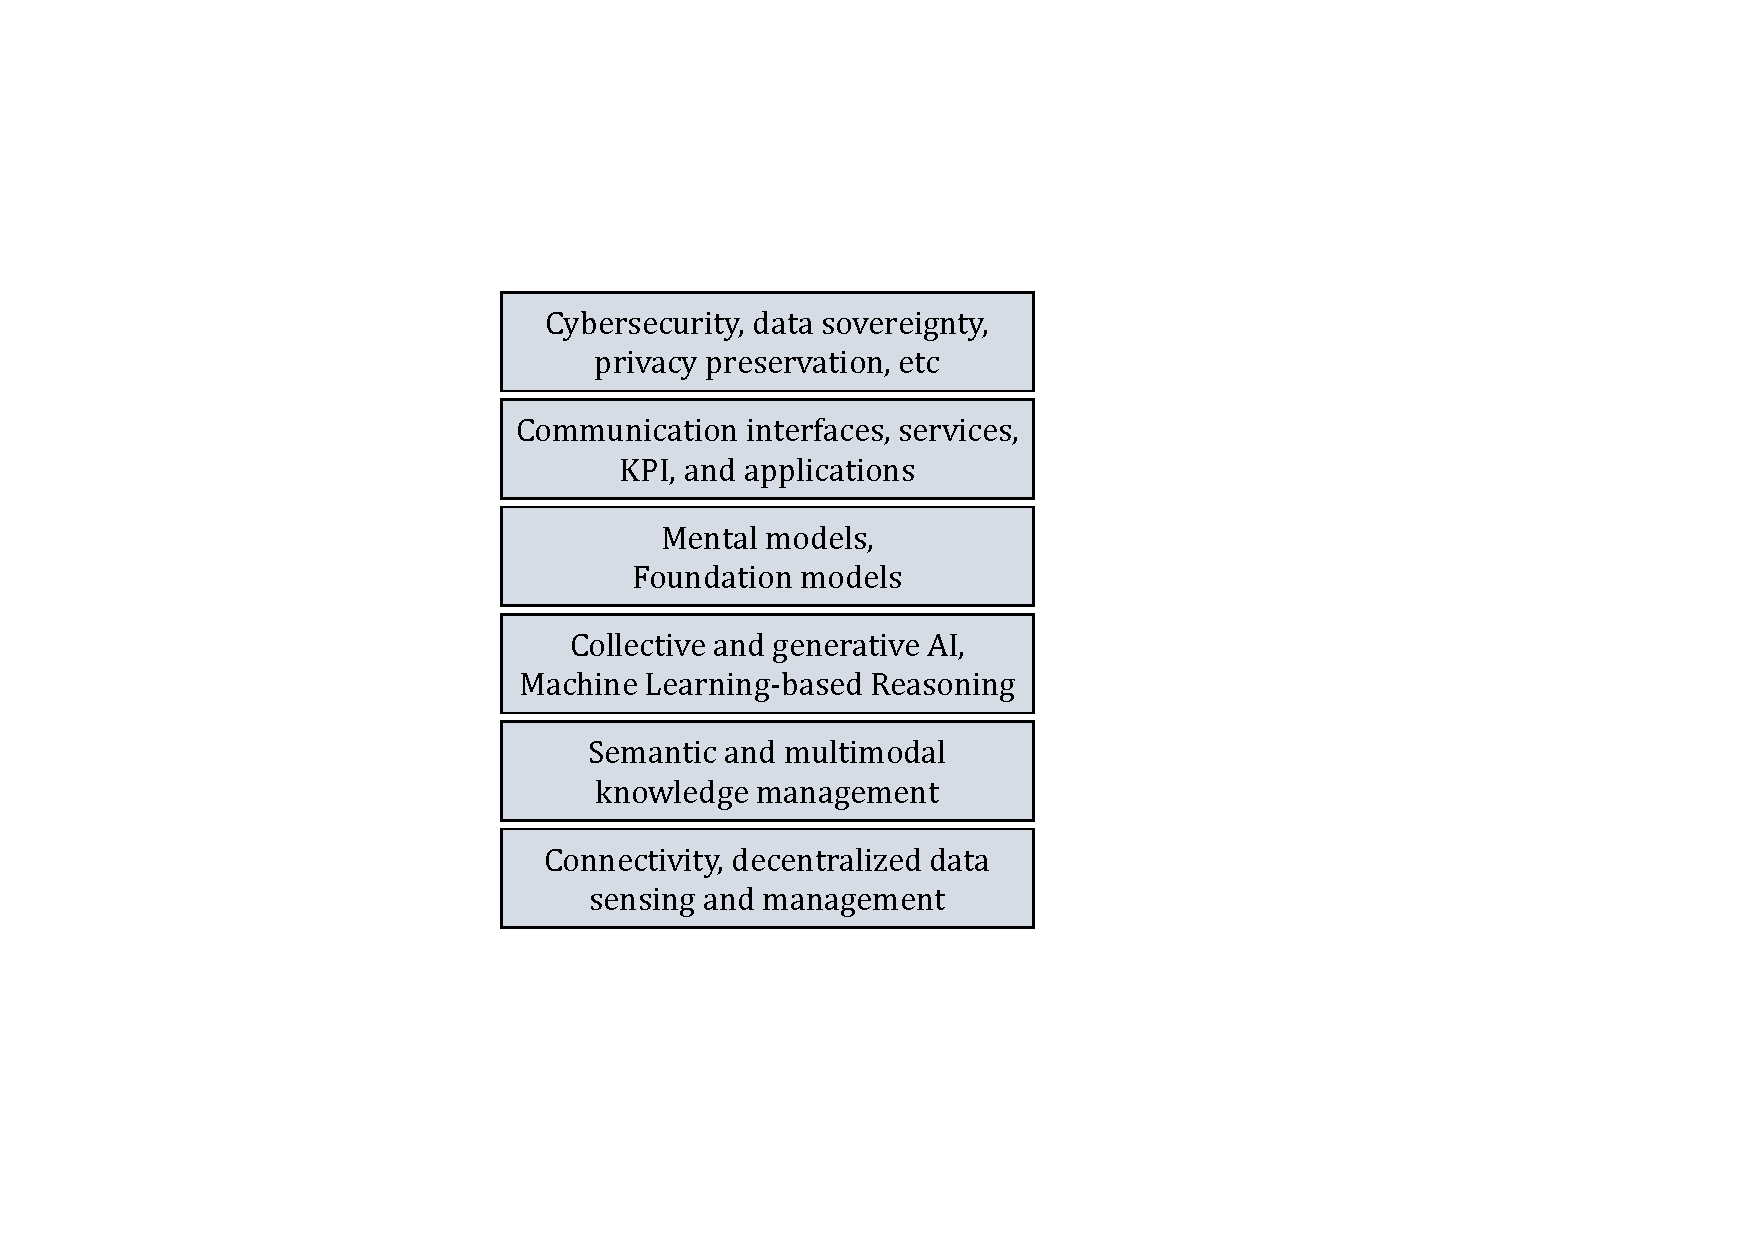
\includegraphics[height=0.6\columnwidth]{images/DT.pdf}}
	\caption{Six-layer architecture of our digital twin. Bottom = 1. layer. Top = 6. layer. 5G connectivity is in the 1. layer. Monitoring, simulation$\slash$extended reality$\slash$Metaverse, and visualization services as well as the computation of Key Performance Indexes (KPI) are carried out in the 5. layer. }
	\label{fig:DT}
\end{figure}

\begin{figure}[b]
	\centerline{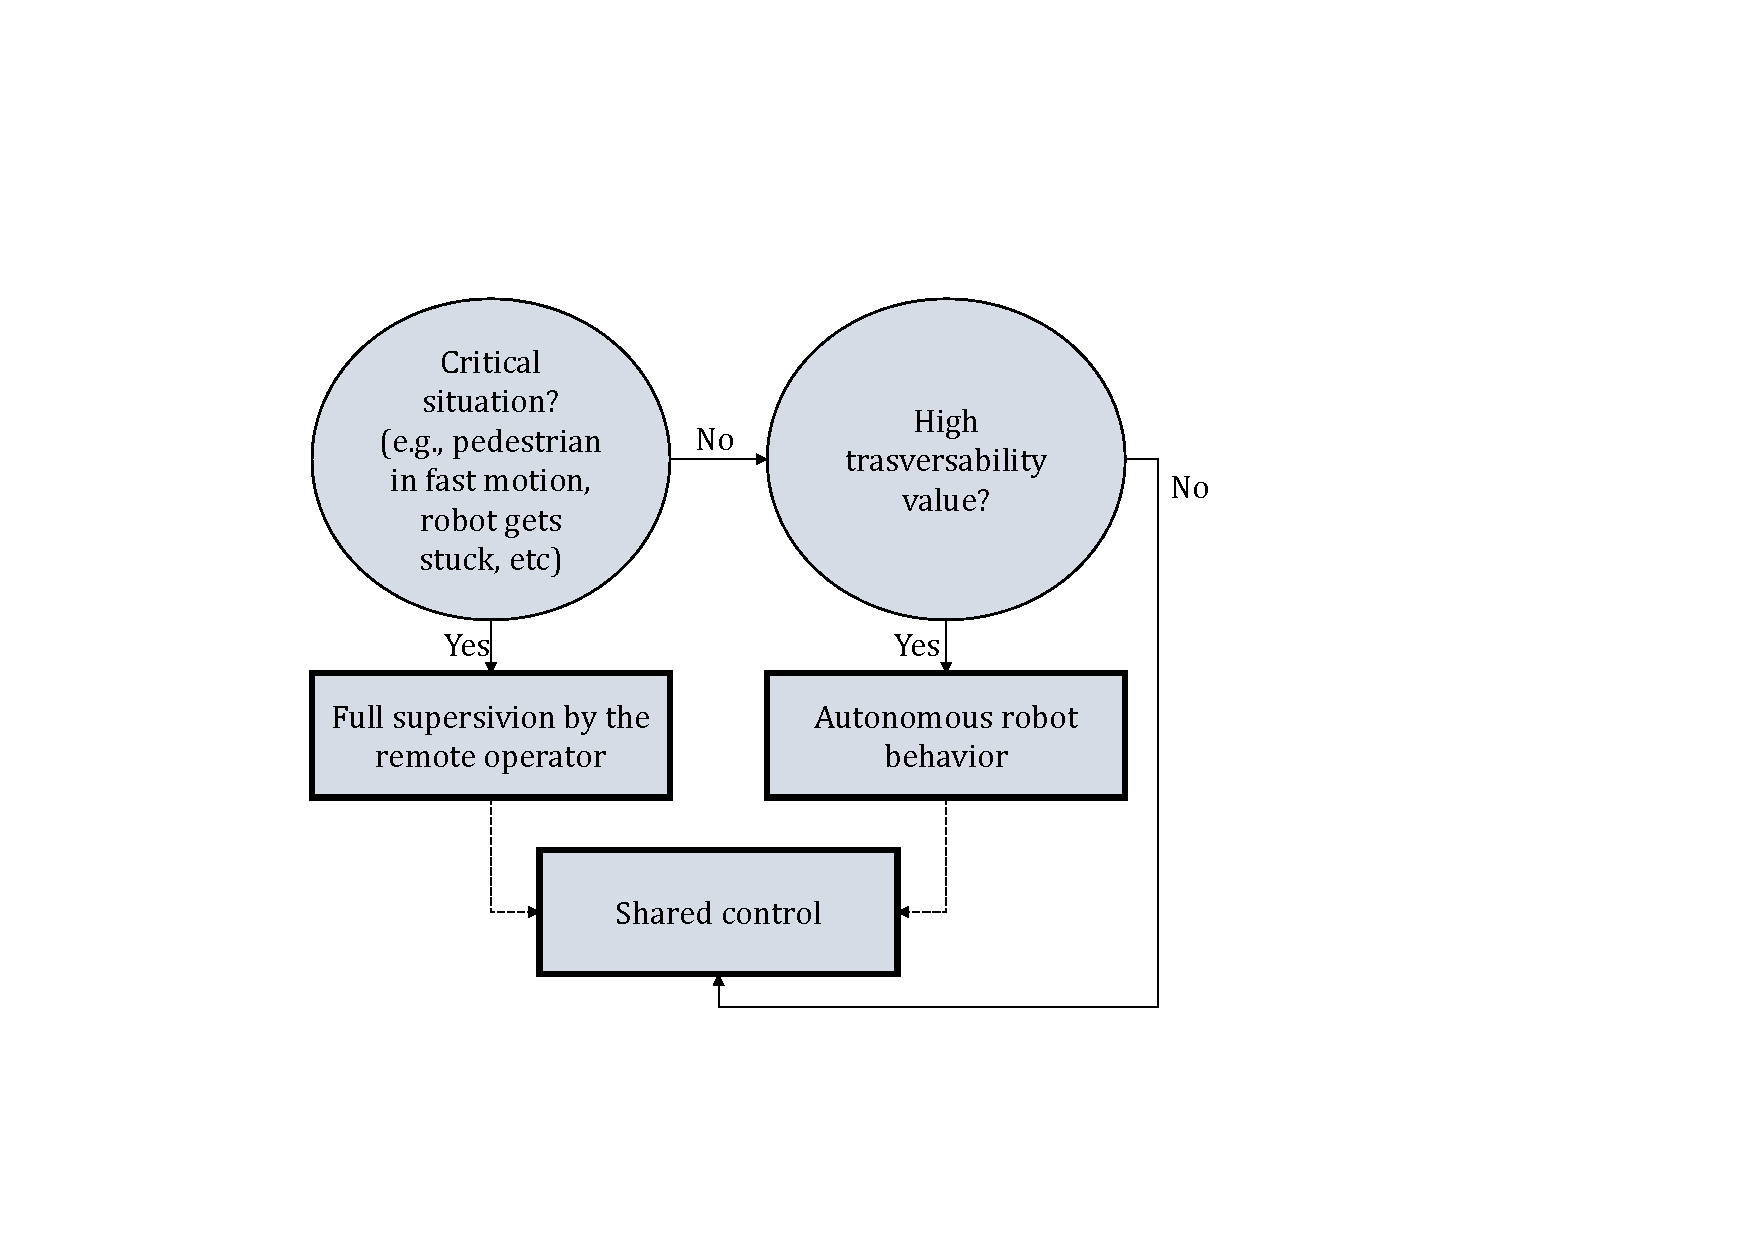
\includegraphics[width=0.7\columnwidth]{images/statemachine.pdf}}
	\caption{Simplified overview of the multiple modes for remote control }
	\label{fig:statemachine}
\end{figure}


A traversability map  contains pairs of linear traversability value $\mu \in [0,1]$  and angular traversability value $\nu\in [0,1]$ for each position on the terrain. A traversability value close to one indicates that a navigation is possible whereas a value close to zero means that the robot  gets stuck \cite{wayfast}. Instead of handling two scalars, the linear and angular traversability values can be combined to yield 
\begin{equation}
	\alpha = \frac{\lambda_1 \mu + \lambda_2 \nu}{2}
\end{equation}
with the weighting coefficients $\lambda_1 \in [0,1]$ and $\lambda_2 \in [0,1]$. Observe that $\alpha \in [0,1]$, too. $\mu = 0$ and $\nu = 0$ together lead  to $\alpha = 0$. Hence, the scalar $\alpha$ can be used to characterize the traversability, as employed in Fig. \ref{fig:architecture} for control purposes.

   \begin{figure}[ht]
	\vspace{0.2cm}
	\centerline{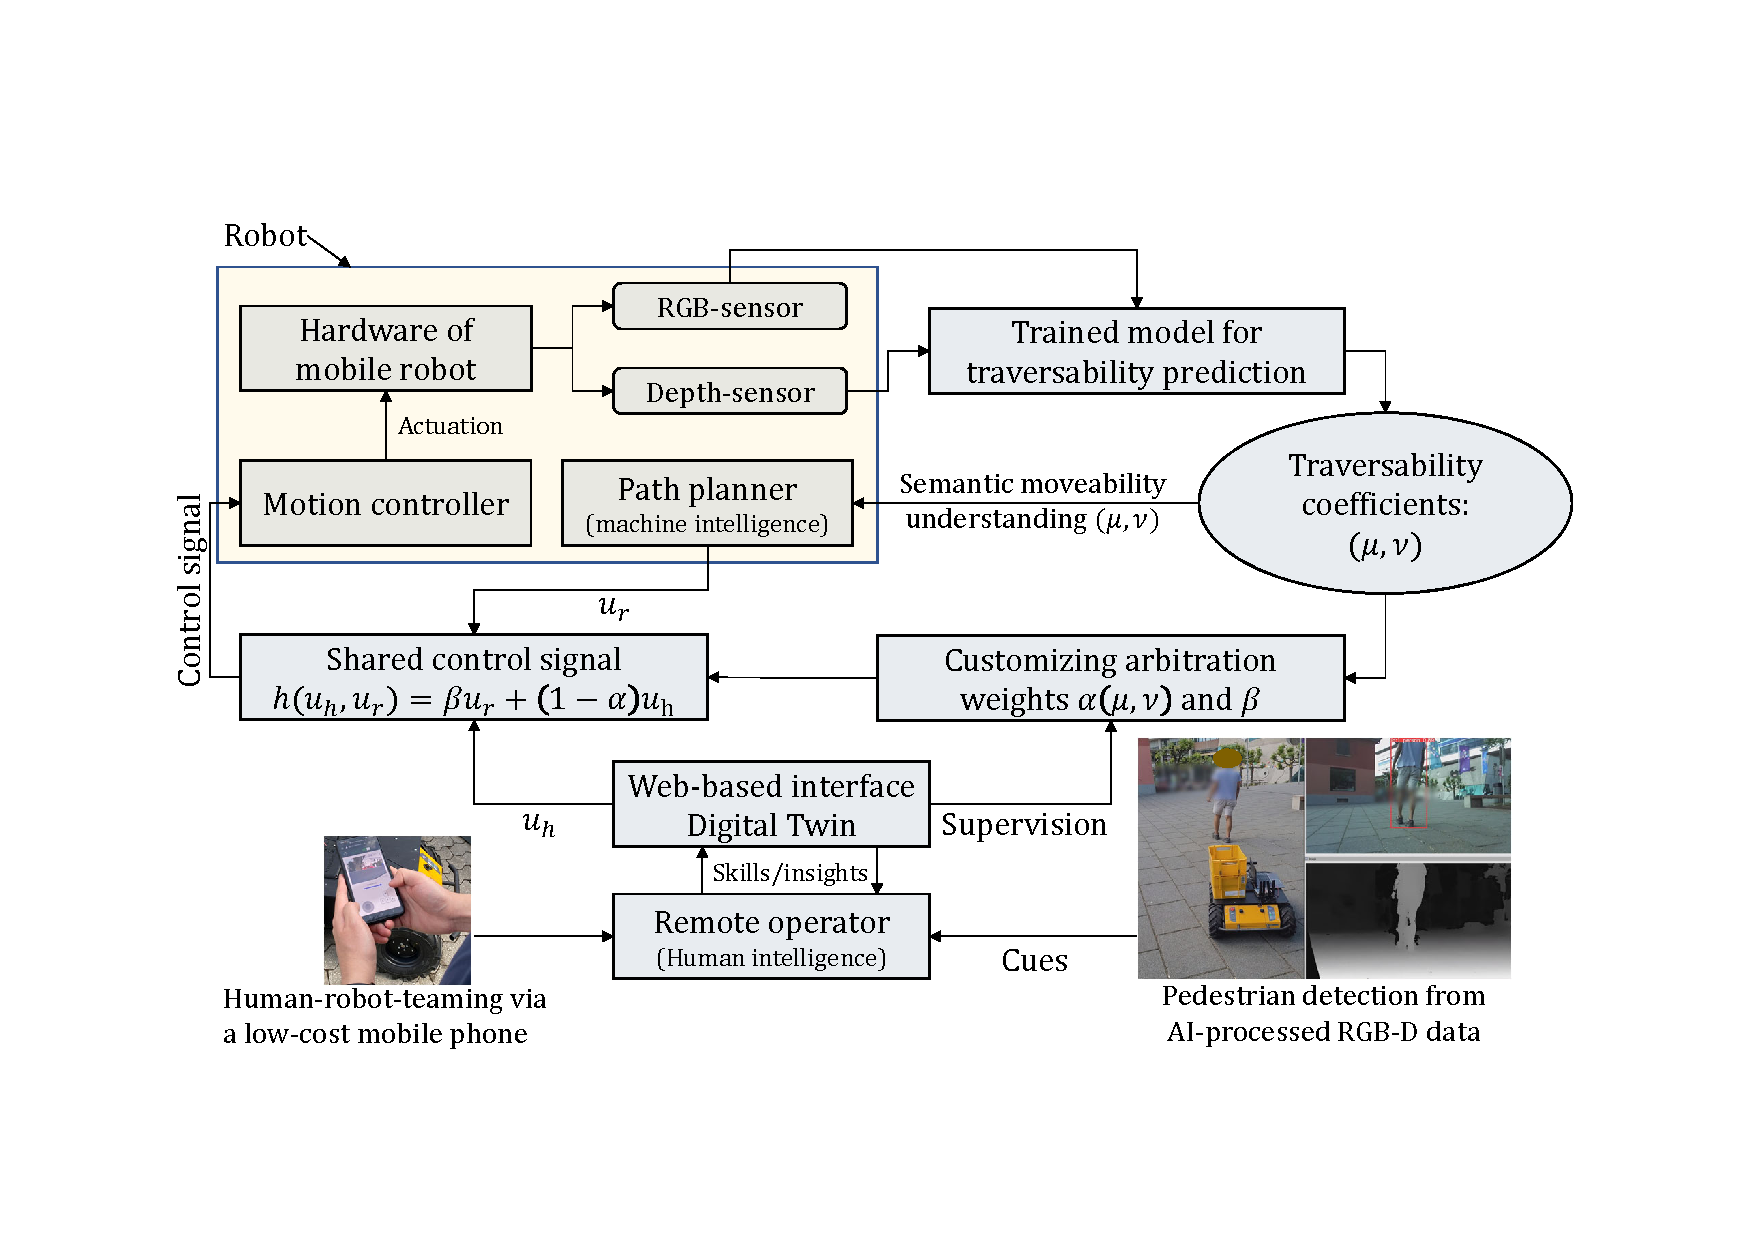
\includegraphics[width=0.95\columnwidth]{images/transversability2.pdf}}
	\caption{Shared control scheme for human-robot teaming (bottom left)}
	\label{fig:architecture}
\end{figure}
\subsection{Autonomous robot behavior without human intervention}
Conditions for a full robot autonomy to happen are that the arbitration variable $\beta=1$ and $\alpha\rightarrow 1$ in 	Fig. \ref{fig:architecture} and Fig. \ref{fig:statemachine}. As a result, the control velocity $h$ is essentially the output of the motion planner of the  robot $u_r$ (see Fig. \ref{fig:architecture}). It is worth to note that the path planner takes advantage of the traversability values to plan a collision free path that safely guides  the robot to the desired goal without human intervention.  Such a path planner can be the Dynamic Window Approach or  Rapidly-Exploring Random Tree scheme  \cite{leung2022hybrid} to cite a few.

\subsection{Full robot supervision by the human operator}
Trained classification models employ images to detect the presence of critical obstacles, such as pedestrians (see Fig. \ref{fig:architecture}), interpret their behavior, and inform the operator using cues, as depicted on the right-hand-side of Fig. \ref{fig:architecture}. Methods for behavior identification based upon graph neural networks are suitable to this end \cite{jang2024multi}. In Fig. \ref{fig:architecture}, RGB and depth data from a state-of-the-art Stereolabs ZED 2i stereo camera sensor (see 	Fig. \ref{fig:userapp}) are forwarded to a pre-trained YOLOv8 model for pedestrian detection (position and orientation). The operator is also aware of potential obstacles around the robot  through visual feedback. To manage the situation, the operator takes over the full control of the robot ($\beta = 0$ and $\alpha = 0$), in which case the operator input (i.e., $h=u_h$, see Fig. \ref{fig:architecture}) is directly forwarded to the motion controller as commanded velocity.

\subsection{Shared control between operator and robot}
In this control mode, the velocity $u_h$ issued by the human operator  is superimposed on top of the velocity $u_r$ generated by the motion planner (note that $\beta = 1$) to yield the  total commanded velocity.  The lower the  value of $\alpha$, the higher the weighting of the contribution  of $u_h$ to the total velocity $h$ (see Fig. \ref{fig:architecture}). If the operator is otherwise engaged ($u_h=0$), the robot evolves autonomously ($h=u_r$). Once the operator is informed or sees that the robot gets stuck ($\alpha \rightarrow 0$), the operator can intervene ($h\approxeq u_r + u_h$) and skillfully sustain the safe and successful navigation of the mobile robot. 
\subsection{Challenges and outlooks}
The ping measured from operator device to the web app averages around 10 ms (local network) and depends on the distance and signal strength. 
Jerking of the camera image can be perceived with greater latency. To improve this, the image resolution and the distance to the robot can be reduced. The model in \cite{wayfaster} takes 320 $\times$ 180 pixels as input. Further improvements could be archived through different encoding methods.
An approach with WebRTC should be evaluated and compared \mbox{against the web video server.}



\section{CONCLUSIONS}
This paper has introduced different modes for the flexible and strengthened remote control of a mobile robot for collaborative navigation purposes. The proposed  shared control fosters human-robot-teaming and supports the continuum between the full supervision of the robot motion using human intelligence  and the autonomous robot behavior based upon a semantic-aware machine intelligence (i.e., self-supervised prediction of traversability values). The approach can support a wide range of outdoor and indoor applications and provides many benefits to the human operator. These include the relaxation of attention requirements, enhanced navigation and immersion experience through digital twins. The approach is suitable for  \mbox{wheeled and also e.g. legged mobile robots.}

\addtolength{\textheight}{-12cm}   % This command serves to balance the column lengths
                                  % on the last page of the document manually. It shortens
                                  % the textheight of the last page by a suitable amount.
                                  % This command does not take effect until the next page
                                  % so it should come on the page before the last. Make
                                  % sure that you do not shorten the textheight too much.

%%%%%%%%%%%%%%%%%%%%%%%%%%%%%%%%%%%%%%%%%%%%%%%%%%%%%%%%%%%%%%%%%%%%%%%%%%%%%%%%



%%%%%%%%%%%%%%%%%%%%%%%%%%%%%%%%%%%%%%%%%%%%%%%%%%%%%%%%%%%%%%%%%%%%%%%%%%%%%%%%



%%%%%%%%%%%%%%%%%%%%%%%%%%%%%%%%%%%%%%%%%%%%%%%%%%%%%%%%%%%%%%%%%%%%%%%%%%%%%%%%




\begin{thebibliography}{99}

\bibitem{wayfast} M. V. Gasparino et al., "WayFAST: Navigation With Predictive Traversability in the Field," in IEEE Robotics and Automation Letters, vol. 7, no. 4, pp. 10651-10658, Oct. 2022, doi: 10.1109/LRA.2022.3193464.
\bibitem{leung2022hybrid}Leung, T., Ignatyev, D. \& Zolotas, A. Hybrid terrain traversability analysis in off-road environments. {\em 2022 8th International Conference On Automation, Robotics And Applications (ICARA)}. pp. 50-56 (2022)
\bibitem{endo2024benchnav}Endo, M., Honda, K. \& Ishigami, G. BenchNav: Simulation Platform for Benchmarking Off-road Navigation Algorithms with Probabilistic Traversability. {\em IEEE ICRA 2024 Workshop on Resilient Off-road Autonomy}. (2024)
%\bibitem{BADGR} G. Kahn, P. Abbeel and S. Levine, "BADGR: An Autonomous Self-Supervised Learning-Based Navigation System," in IEEE Robotics and Automation Letters, vol. 6, no. 2, pp. 1312-1319, April 2021, doi: 10.1109/LRA.2021.3057023.
\bibitem{wayfaster} M. V. Gasparino et al., "WayFASTER: a Self-Supervised Traversability Prediction for Increased Navigation Awareness," Feb. 2024 arXiv.
\bibitem{frey2024roadrunner}Frey, J., Khattak, S., Patel, M., Atha, D., Nubert, J., Padgett, C., Hutter, M. \& Spieler, P. RoadRunner–Learning Traversability Estimation for Autonomous Off-road Driving. {\em Preprint ArXiv:2402.19341}. (2024)
\bibitem{muhamad2024robust}Muhamad, F., Kim, J. \& Park, J. Robust Traversability Prediction Using Multiple Costs for Quadruped Robot in Random Terrains. {\em IEEE Access}. (2024)
\bibitem{huang2024evaluation}Huang, C., Chou, S., Liou, L., Moy, N., Wang, C., Wang, H., Ahn, C., Huang, C. \& Yu, L. An Evaluation Framework of Human-Robot Teaming for Navigation Among Movable Obstacles via Virtual Reality-Based Interactions. {\em IEEE Robotics And Autom. Letters}. (2024)
\bibitem{husky}"Husky Unmanned Ground Vehicle," Clearpath, https://clearpathrobotics.com/husky-unmanned-ground-vehicle-robot/ (accessed Aug. 9, 2024).

\bibitem{phri} M. Selvaggio, M. Cognetti, S. Nikolaidis, S. Ivaldi and B. Siciliano, "Autonomy in Physical Human-Robot Interaction: A Brief Survey," in IEEE Robotics and Automation Letters, vol. 6, no. 4, pp. 7989-7996, Oct. 2021, doi: 10.1109/LRA.2021.3100603.



\bibitem{kapic} Zinaid Kapić, Aladin Crnkić, Edin Mujčić and Jasna Hamzabegović, "A web application for remote control of ROS robot based on WebSocket protocol and Django development environment", in IOP Conf. Ser.: Mater. Sci. Eng. 1208 012035, 2021, doi: 10.1088/1757-899X/1208/1/012035.
\bibitem{dinodi} D. D. Rajapaksha et al., "Web Based User-Friendly Graphical Interface to Control Robots with ROS Environment," 2021 6th International Conference on Information Technology Research (ICITR), Moratuwa, Sri Lanka, 2021, pp. 1-6, doi: 10.1109/ICITR54349.2021.9657337.
\bibitem{rosbridgeOkState} Crick, C., Jay, G., Osentoski, S., Pitzer, B., and Jenkins, O. C. "Rosbridge: Ros for non-ros users" in Rob. Research, Springer, 2017.
\bibitem{rosbridgeSuite}"rosbridge\_suite," rosbridge suite - ROS Wiki, http://wiki.ros.org/rosbridge\_suite (accessed Aug. 9, 2024).

\bibitem{walker2024cyber}Walker, M., Gramopadhye, M., Ikeda, B., Burns, J. \& Szafir, D. The Cyber-Physical Control Room: A Mixed Reality Interface for Mobile Robot Teleoperation and Human-Robot Teaming. {\em Proceedings Of The 2024 ACM/IEEE International Conference On Human-Robot Interaction}. pp. 762-771 (2024)
\bibitem{flask}"Flask," User’s Guide, https://flask.palletsprojects.com/en/3.0.x/
\bibitem{bootstrap}"Introduction," Bootstrap, https://getbootstrap.com/docs/5.3/getting-started/introduction/ (accessed Aug. 9, 2024).
\bibitem{jang2024multi}Jang, S., Lee, H., Kim, W., Lee, J., Woo, S. \& Lee, S. Multi-scale Structural Graph Convolutional Network for Skeleton-based Action Recognition. {\em IEEE Trans. On Circuits \& Syst. For Video Techn.}(2024)




% \bibitem{controlpriority}"Interfacing with Husky," Clearpath, https://www.clearpathrobotics.com/assets/guides/melodic/husky/InterfacingWithHusky.html (accessed Aug. 9, 2024).
% \bibitem{energy} https://ieeexplore.ieee.org/stamp/stamp.jsp?tp=&arnumber=9808373
% \bibitem{seamless} https://ieeexplore.ieee.org/stamp/stamp.jsp?tp=&arnumber=9372861






\end{thebibliography}




\end{document}
